\documentclass{article}
\usepackage{graphicx}
\usepackage{hyperref}
\usepackage{titlesec}
\usepackage[T1]{fontenc}
\usepackage{amsmath}
\usepackage{subfigure}

\usepackage[margin=2cm]{geometry} % set 2cm margins

\linespread{1.4}

\hypersetup{
  colorlinks = true,
  linkcolor  = blue,
  citecolor  = blue,
  urlcolor   = blue
}

\titleformat{\section}
  {\fontsize{33}{54}\selectfont\bfseries}
  {\thesection\hspace{10pt}}
  {0pt}
  {}
\renewcommand{\figurename}{Slika}
\begin{document}


\title{\fontsize{36}{22}\selectfont Dva topa}
\author{\fontsize{14}{18}\selectfont Lazar Stanojević Vasilije Todorović Vukašin Radić}
\date{8. Maj 2023.}
\maketitle    


\newpage

\begin{center}
\textbf{\huge Sadržaj}
\end{center}

\hrule

\bigskip

\textbf{\Large \hyperref[sec:uvod]{1. Uvod}} \dotfill 3

\medskip

\textbf{\Large \hyperref[sec:modelovanje]{2. Modelovanje problema}} \dotfill 4

\medskip

\textbf{\Large \hyperref[sec:sudar]{3. Sudar}} \dotfill 7

\medskip

\textbf{\hspace{0.5cm} \Large \hyperref[sec:sudarnize]{3.1 Sudar iznad nižeg brda}} \dotfill 9

\medskip

\textbf{\hspace{0.5cm} \Large \hyperref[sec:sudargraf]{3.2 Grafički prikaz sudara}} \dotfill 10

\medskip

\textbf{\Large \hyperref[sec:literatura]{Literatura}} \dotfill 11

\bigskip

\hrule

\bigskip

\newpage

\section{\huge Uvod}\label{sec:uvod}
\fontsize{14}{14}\selectfont
Ovaj problem je dobio ime po dva topa koja se nalaze na dva različita brda. Oba brda imaju svoju visinu, dalje u tekstu $h_1$ i $h_2$, respektivno s leva na desno. Bez umanjenja opštosti pretpostavićemo da je levo brdo visoko bar koliko i desno brdo, tj. da je $h_1 \geq h_2$.
\newline
Brda se nalaze na rastojanju $d$ jedno od drugog. Topovi nišane jedan prema drugom i istovremeno ispaljuju đule sa nekim početnim brzinama, moguće različitim. 
\newline

\begin{figure}[h]
  \centering
  \begin{minipage}[b]{0.45\linewidth}
    \centering
    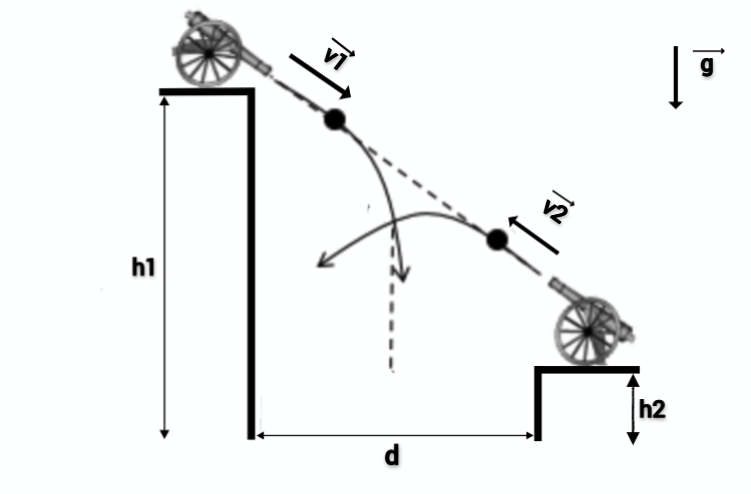
\includegraphics[width=\linewidth]{omm_slika.png}
    \caption{Postavka problema.}
    \label{fig:image1}
  \end{minipage}
  \hspace{0.5cm}
  \begin{minipage}[b]{0.45\linewidth}
    \centering
    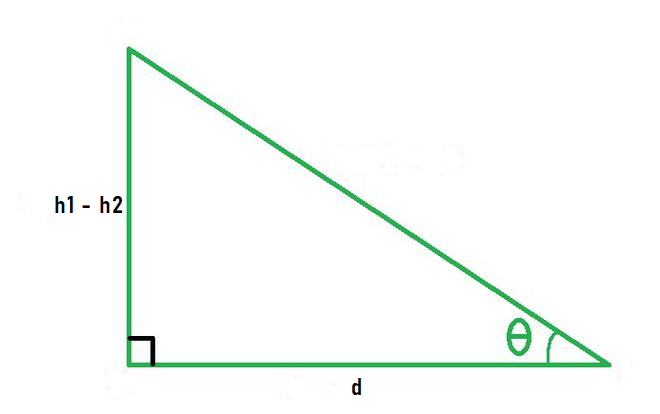
\includegraphics[width=\linewidth]{trougao_slika.png}
    \caption{Ugao ispaljivanja.}
    \label{fig:image2}
  \end{minipage}
  \label{fig:my_images}
\end{figure}

Na slici 1 se vidi početna postavka problema. Naš zadatak u daljem radu će biti da pokažemo da se đuladi moraju sudariti, bez obzira na visine i rastojanje brda, kao i početne brzine pod kojima su ispaljena.
\newline
Takođe, ispitaćemo i pod kojim uslovima će se ona sudariti na visini većoj od visine nižeg brda, i prikazati lokacije sudara za fiksirane pozicije, u zavisnosti od početnih brzina.

\newpage
\section{\huge Modelovanje problema}\label{sec:modelovanje}
Problem spada u klasu problema kosog hica, kombinovanog sa nekom vrstom hica naniže.
Pre samog modelovanja, a u cilju preciznijeg definisanja matematičkog modela, uvešćemo određene pretpostavke koje će važiti za naš model.
\newline
\begin{enumerate}
  \item Koordinate sa kojeg se ispaljuje prvo đule su $(0, h_1)$
  \item Koordinate sa kojeg se ispaljuje drugo đule su $(d, h_2)$
  \item Đuladi se mogu predstaviti kao materijalne tačke
  \item U svakom trenutku t, možemo izračunati koordinate đuladi
  \item $x_1(t)$ i $y_1(t)$ odgovaraju x i y koordinatama prvog đuleta, u trenutku $t$
  \item $x_2(t)$ i $y_2(t)$ odgovaraju x i y koordinatama drugog đuleta, u trenutku $t$
  \item Ceo eksperiment se odvija u vakuumu
  \item Jačina sile zemljine teže ne zavisi od visine, već je svuda $g = 9.81 \mathrm{m/s^2}$
  \item Funkcije $x_1(t), y_1(t), x_2(t)$ i $y_2(t)$ su dva puta neprekidno diferencijabilne funkcije
  \item Početne brzine kojima se đulad ispaljuju su $v_1$ i $v_2$, respektivno
  \item Između topova se nalazi provalija, odnosno dno nije ograničeno y osom
  \newline
\end{enumerate}
Kako se topovi međusobno nišane, uglove pod kojima će đulad biti ispaljena možemo direktno izračunati na osnovu pozicije topova. Označićemo sa $\theta$ ugao pod kojim desni top nišani levi.
\newline
Sada iz pravouglog trougla direktno sledi da je 
\begin{align}
    \theta = \arctan( \frac{h1 - h2}{d}) \notag
\end{align}
Ugao pod kojim levi top nišani desni je 90\textdegree - $\theta$.
\newpage

Sada imamo da je: 
    \begin{align}
    v_{x1} = v_1\cdot\cos(\theta),  \quad v_{y1} = v_1 \cdot \sin(\theta) \notag  
    \end{align}
    \begin{align}
    v_{x2} = v_2 \cdot \cos(\theta), \quad v_{y2} = v_2 \cdot \sin(\theta) \notag
    \end{align}    
Na đulad deluje sila zemljine teže u negativnom smeru, koju možemo posmatrati kao negativno ubrzanje.
Zbog toga imamo da je:
\begin{align}
    y_1''(t) = -g \quad i \quad y_2''(t) = -g \notag 
\end{align}

Integraljenjem ovih jednačina na segmentu (0, t] dobijamo da je:
\begin{align}
      y_1'(t) = -g \cdot t + C_1, \quad i \quad y_2'(t) = -g \cdot t + C_2  \tag {1}
\end{align}
Kako je $y_1'(0) = -v_{y1}$ i $y_2'(0) = v_{y2}$, možemo odrediti konstante $C_1$ i $C_2$. 
\newline Zamenom $t = 0$ u (1) dobijamo:
\begin{align}
  C_1=-v_{y1} \quad i \quad C_2=v_{y2}  \tag {2}
\end{align}
Na osnovu (1) i (2) dobijamo: 
\begin{align}
        y_1'(t) = -g \cdot t - v_{y1} \quad i \quad y_2'(t) = -g \cdot t + v_{y2} \tag {3}
\end{align}
Ponovo možemo da integralimo ove jednačine, i time dobijamo:
\begin{align}
        y_1(t) = - v_{y1} \cdot t - g \cdot \frac{t^2}{2} + C_3 , \quad y_2(t) =v_{y2} \cdot t - g \cdot \frac{t^2}{2} + C_4 \tag {4}
\end{align}
Kako se prvo đule na početku nalazi na visini $h_1$, imamo da je $y_1(0) = h_1$ iz čega sledi $C_3=h_1$. 
\newline
Zamenom $C_3$ u (4) dobijamo:
\begin{align}
    y_1(t) = h_1 - v_{y1} \cdot t - g \cdot \frac{t^2}{2} \tag {5}
\end{align}
Kako se drugo đule na početku nalazi na visini $h_2$, analogno se dobija:
\begin{align}
    y_2(t) = h_2 + v_{y2} \cdot t - g \cdot \frac{t^2}{2} \tag {6}
\end{align}
Na osnovu početnih uslova, imamo: 
\begin{align}
    x_1'(0) = v_{x1} = v_1 \cdot \cos(\theta) \quad i \quad x_2'(0) = -v_{x2} = - v_2 \cdot \cos(\theta) \notag 
\end{align}
Integraljenjem dobijamo: 
\begin{align}
    x_1(t) = v_1 \cdot \cos(\theta) \cdot t + C_5 \quad i \quad x_2(t) =  -v_2 \cdot \cos(\theta) \cdot t + C_6 \tag {7}
\end{align}
Iz početnih pozicija imamo da je $x_1(0) = 0$ i $x_2(0) = d$ iz čega sledi da je $C_5 = 0$ i $C_6 = d$, zamenom $t = 0$ u (7).
\newline
\newline
Konačno dobijamo:
\begin{align}
    x_1(t) = v_1 \cdot \cos(\theta) \cdot t \quad i \quad x_2(t) = d - v_2 \cdot \cos(\theta) \cdot t  \tag {8}
\end{align}
Kretanja đuladi matematički možemo opisati sledećim formulama:
\begin{align}
    x_1(t) = v_1 \cdot \cos(\theta) \cdot t, \quad y_1(t) = h_1 - v_1 \cdot \sin(\theta) \cdot t - g \cdot \frac{t^2}{2} \tag {9}
\end{align}
\begin{align}
    x_2(t) = d - v_2 \cdot \cos(\theta) \cdot t , \quad
    y_2(t) = h_2 + v_2 \cdot \sin(\theta) \cdot t - g \cdot \frac{t^2}{2} \tag {10}
\end{align}
$y_1(t)$ i $y_2(t)$ su dobijene zamenom $v_{y1} = v_1 \cdot \sin(\theta)$ i $v_{y2} = v_2 \cdot \sin(\theta)$ u (5) i (6), respektivno.
\newpage
\section{\huge Sudar}\label{sec:sudar}
U narednom delu želimo dokazati da će se đuladi uvek sudariti, bez obzira na parametre u modelu. Ideja je da pokažemo da se oni nikad neće mimoići, tj. da ako im se poklope $x$ koordinate, poklopiće im se i $y$.
\newline
\newline Kako bismo dobili vreme za koje će im se $x$ koordinate poklopiti, izjednačićemo jednačine za $x$ koordinate iz (9) i (10). Dobijamo: 
\begin{align}
    v_1 \cdot \cos(\theta) \cdot t = d - v_2 \cdot \cos(\theta) \cdot t \notag
\end{align}
Iz ove jednakosti izražavamo $t$, i dobijamo:
\begin{align}
    t = \frac{d}{\cos(\theta) \cdot (v_1 + v_2)}        \tag{11}
\end{align}
Pokazaćemo da će se za dobijeno vreme $t$ poklopiti i $y$ koordinate.
Zamenom dobijenog $t$ u jednačine za izračunavanje $y$ koordinata iz (9) i (10) dobijamo:
\begin{align}
    y_1 = h_1 - v_1 \cdot \sin(\theta) \cdot \frac{d}{\cos(\theta) \cdot (v_1 + v_2)} - \frac{g}{2} \cdot \frac{d^2}{\cos(\theta)^2 \cdot (v_1 + v_2)^2} \nonumber \\ 
    y_2 = h_2 + v_2 \cdot \sin(\theta) \cdot \frac{d}{\cos(\theta) \cdot (v_1 + v_2)} - \frac{g}{2} \cdot \frac{d^2}{\cos(\theta)^2 \cdot (v_1 + v_2)^2} \notag
\end{align}
Kako iz trougla sa slike 2 imamo da je $h_1 - h_2 = \tan(\theta) * d$, proširivanjem desne strane sa $v_1 + v_2$ dobijamo:
\begin{align}
    h_1 - h_2 = \tan(\theta) \cdot d \cdot \frac{v_1 + v_2}{v_1 + v_2} \notag
\end{align}
Odatle sledi da je:
\begin{align}
    h_1 - h_2 = v_1 \cdot \sin(\theta) \cdot d \cdot  \frac{1}{\cos(\theta) \cdot (v_1 + v_2)} + v_2 \cdot \sin(\theta) \cdot d \cdot \frac{}{\cos(\theta) \cdot (v_1 + v_2)} \notag
\end{align}
Prebacivanjem odgovarajućih sabiraka na odgovarajuće strane iz prethodne jednakosti, dobijamo:
\begin{align}
    h_1 -v_1 \cdot \sin(\theta) \cdot d \cdot  \frac{1}{\cos(\theta) \cdot (v_1 + v_2)} = h_2 + v_2 \cdot \sin(\theta) \cdot d \cdot \frac{1}{\cos(\theta) \cdot (v_1 + v_2)} \notag
\end{align}
Konačno, oduzimanjem $\frac{g}{2} \cdot \frac{d^2}{\cos(\theta)^2 \cdot (v_1 + v_2)^2}$ od obe strane jednakosti, dobijamo $y_1 = y_2$, odnosno za dato $t$, i $y$ koordinate će im biti iste.
\newline
\newline
Ovim smo pokazali da kad god se $x$ koordinate đuladi poklope, poklopiće im se i $y$ koordinate, odnosno da će doći do sudara. Kako se oni kreću u suportnim smerovima, a nema ničega što ih usporava ili zaustavlja po $x$ osi, oni će se svakako u nekom momentu susresti po $x$ koordinatama iz čega sledi da će im se sigurno poklopiti i $y$ koordinate, na osnovu prethodno izvedenog.
\newpage
\subsection{\huge Sudar iznad nižeg brda}\label{sec:sudarnize}
U narednom delu želimo da ispitamo pod kojim uslovima će do sudara doći na visini koja je barem visine nižeg brda.
\newline
Kako smo pokazali da će do sudara uvek doći, sada ćemo samo zahtevati da y koordinata sudara bude veća ili jednaka $h_2$ i videti kada će to važiti.
\newline
\newline
Vreme za koje dolazi do sudara dobijamo isto kao i ranije, izjednačavanjem x koordinata. To vreme iznosi:
\begin{align}
    t = \frac{d}{\cos(\theta) \cdot (v_1 + v_2)} \notag
\end{align}
Zamenom $t$ u bilo koju $y$ koordinatu đuladi, dobićemo koordinatu sudara:
\begin{align}
   y_2 = h_2 + v_2 \cdot \sin(\theta) \cdot \frac{d}{\cos(\theta) \cdot (v_1 + v_2)} - \frac{g}{2} \cdot \frac{d^2}{\cos(\theta)^2 \cdot (v_1 + v_2)^2} \notag
\end{align}
Za koordinatu $y_2$ važi da je veća ili jednaka od $h_2$ kada je:
\begin{align}
    v_2 \cdot \sin(\theta) \cdot \frac{d}{\cos(\theta) \cdot (v_1 + v_2)} - \frac{g}{2} \cdot \frac{d^2}{\cos(\theta)^2 \cdot (v_1 + v_2)^2} \geq 0 \notag
\end{align}
Svođenjem na zajednički imenilac, dobijamo:
\begin{align}
    (v_2 \cdot \sin(\theta) \cdot d \cdot \cos(\theta) \cdot (v_1 + v_2) \cdot 2 - g \cdot d^2) / (2 \cdot \cos(\theta) \cdot (v_1 + v_2)) ^ 2  \geq 0 \notag
\end{align}
Kako je imenilac uvek pozitivan, imamo da će uslov važiti kada je ispunjeno da je brojilac pozitivan:
\begin{align}
    v_2 \cdot \sin(\theta) \cdot d \cdot \cos(\theta) \cdot (v_1 + v_2) \cdot 2 - g \cdot d^2 \geq 0 \notag
\end{align}
Prebacivanjem $g \cdot d^2$ na desnu stranu nejednakosti i potom deljenjem cele nejednakosti sa $d$ dobijamo:
\begin{align}
v_2 \cdot \sin(\theta) \cdot \cos(\theta) \cdot 2 \cdot (v_1 + v_2) \geq g \cdot d \notag  
\end{align}
Sada, korišćenjem jednakosti $2 \cdot \sin(\theta) \cdot \cos(\theta) = \sin (2\theta)$, i deljenjem nejednakosti sa time, konačno dobijamo:
\begin{align}
v_2 \cdot (v_1 + v_2) \geq \frac{g \cdot d}{\sin(2\theta)} \tag{12}   
\end{align}
Ovo je uslov koji mora da važi za početne brzine ispaljivanja, kako bi do sudara došlo iznad nižeg brda.
\newpage

\subsection{\huge Grafički prikaz sudara}\label{sec:sudargraf}
Naredne slike generisane su pomoću Matlaba. Na slikama 3, 4 i 5 prikazali smo pozicije sudara đuladi, u zavisnosti od različitih početnih brzina. Skale $y$ ose su različite, radi boljeg pregleda.
\newline
Na slici 6 prikazane su trajektorije đuladi za dve fiksirane početne brzine, kao i pozicija na kojoj će doći do sudara.
\begin{figure}[h]
  \centering
  \begin{minipage}[b]{0.45\linewidth}
    \centering
    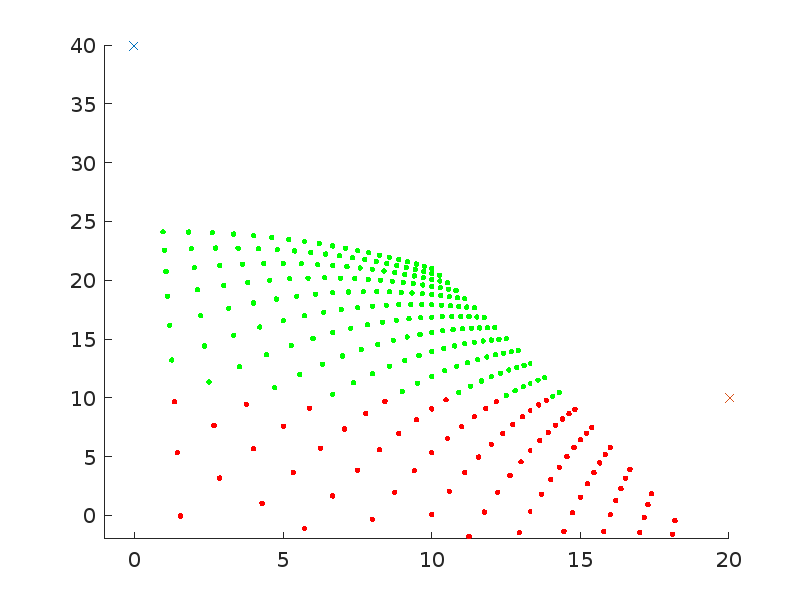
\includegraphics[width=\linewidth]{slika2_omm.png}
    \caption{Grafički prikaz sudara.}
    \label{fig:image3}
  \end{minipage}
  \hspace{0.5cm}
  \begin{minipage}[b]{0.45\linewidth}
    \centering
    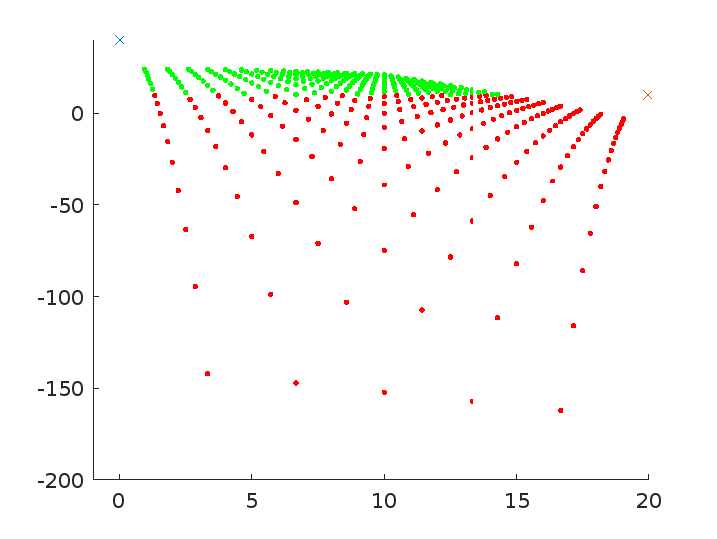
\includegraphics[width=\linewidth]{slika3_omm.png}
    \caption{Grafički prikaz sudara.}
    \label{fig:image4}
  \end{minipage}
  \label{fig:my_images1}
\end{figure}

\begin{figure}[h]
  \centering
  \begin{minipage}[b]{0.45\linewidth}
    \centering
    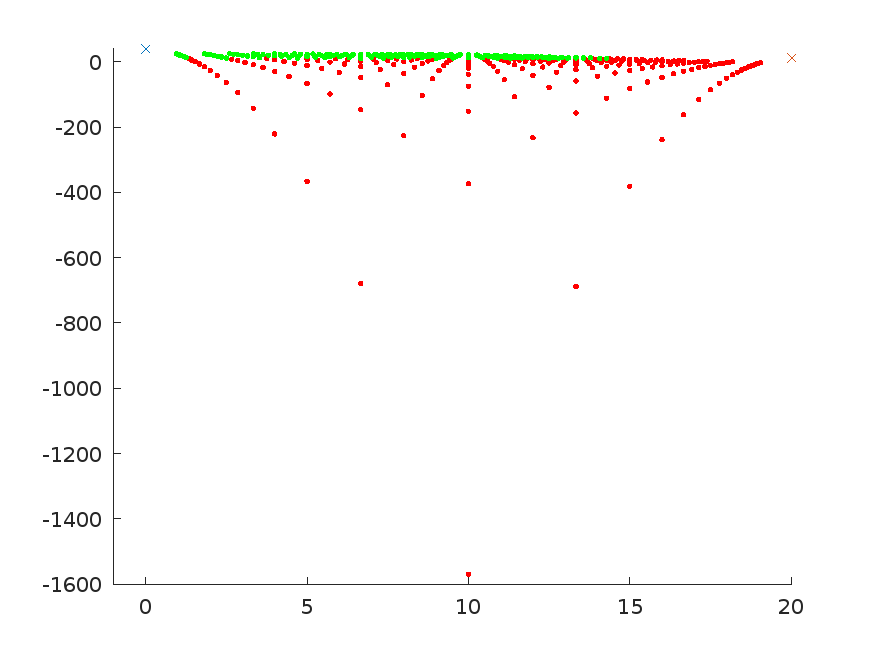
\includegraphics[width=\linewidth]{slika4_omm.png}
    \caption{Grafički prikaz sudara.}
    \label{fig:image5}
  \end{minipage}
  \hspace{0.5cm}
  \begin{minipage}[b]{0.45\linewidth}
    \centering
    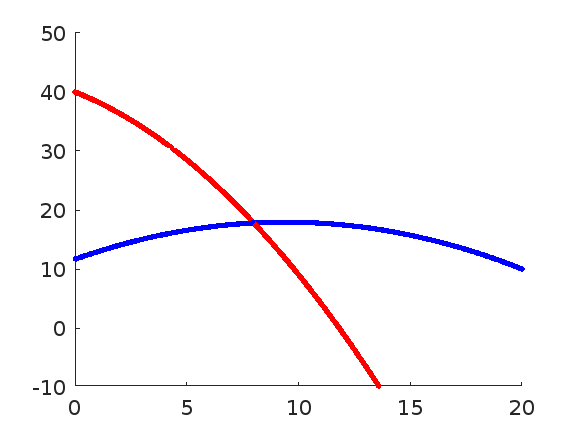
\includegraphics[width=\linewidth]{sudar.png}
    \caption{Trajektorije i sudar đuladi.}
    \label{fig:image6}
  \end{minipage}
  \label{fig:my_images2}
\end{figure}
\newpage


\section{\huge Literatura}\label{sec:literatura}
\begin{enumerate}
  \setcounter{enumi}{0}
  \renewcommand{\labelenumi}{[\arabic{enumi}]}
  \item Milan Dražić, Matematičko modeliranje. Matematički fakultet, Beograd,
2017.
  \item Stranica kursa Osnove matematičkog modeliranja (http://poincare.matf.bg.ac.rs/~zorica.drazic/OMM2023.html)
  \item Osnova za sliku 1 preuzeta sa sajta bartleby.com
\end{enumerate}
\end{document}
